% Quatrième partie : transition numérotée du gabarit Perso.
\setcounter{chapCompteur}{4}
\ChapNumber{\myChapNum}{\hspace*{0.8cm}\LARGE \textbf{Dans Python}}{\hspace*{0.8cm}\small Du tableau à l'application}
\section{Dans un programme Python}

\begin{frame}[t,fragile]{Projeter, exporter ou obtenir une figure depuis un DataFrame}
\vfill
\begin{columns}[T,totalwidth=1.05\textwidth]
\begin{column}{0.56\textwidth}
{\relscale{0.9}
\texttt{df} est un DataFrame pandas~\cite{pandas} : voir \texttt{examples/client\_project/depuis\_pandas.py} (huit essais de soudage synthétiques). Il n'est pas modifié.
\begin{lstlisting}[style=py_style1,numbers=none,basicstyle=\ttfamily\footnotesize,xleftmargin=0pt,breakatwhitespace=false,breakindent=0pt,keepspaces=true]
import dim2dir
projection = dim2dir.project(df)
result = dim2dir.visualize(
    df, output_dir="resultats_pandas",
    outputs=("png", "pdf"))
print(result.files, result.warnings)
\end{lstlisting}
\texttt{projection.occupied}, \texttt{.width} et \texttt{.height} donnent la couverture sans exporter.
}
\end{column}
\begin{column}{0.42\textwidth}
\centering
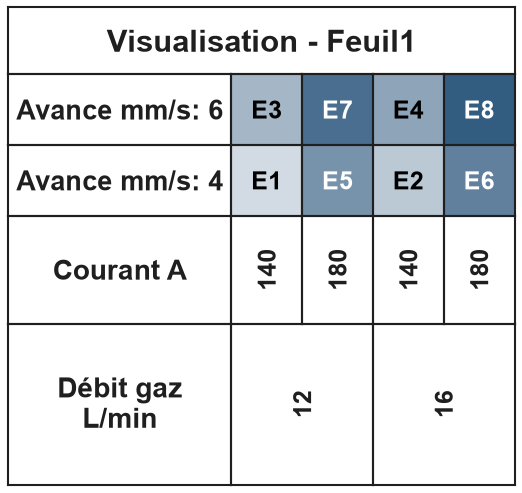
\includegraphics[width=\linewidth,height=0.35\textheight,keepaspectratio]{./_FIG/FIG_Partie_00/client_pandas.png}
\par\vspace{0.2em}
{\footnotesize \texttt{resultats\_pandas/plan\_visu\_Feuil1.png}}
\par\vspace{0.3em}
\raggedright
{\relscale{0.9}
Dans un notebook, terminer la cellule par \texttt{fig}. L'appel retourne une figure matplotlib~\cite{matplotlib}, sans affichage automatique.
\begin{lstlisting}[style=py_style1,numbers=none,basicstyle=\ttfamily\footnotesize,xleftmargin=0pt,breakatwhitespace=false,breakindent=0pt,keepspaces=true]
fig = dim2dir.figure(df)
fig
\end{lstlisting}
}
\end{column}
\end{columns}
\note{Adaptation de examples/client_project/depuis_pandas.py : df = welding_plan(), trois facteurs à deux niveaux, ici style par défaut comme sur la figure fournie. L'exemple utilise HERE / "resultats_pandas" pour rendre le dossier indépendant du dossier courant. L'API accepte aussi un chemin xlsx, une liste de dictionnaires ou un dictionnaire de listes. project n'alloue pas de grille dense.}
\vfill
\end{frame}

\begin{frame}[t]{Un objet Style règle palette, police et tailles}
% [DEVELOPPE: tableaux des champs]
\vfill
{\footnotesize\setlength{\tabcolsep}{2.5pt}
\begin{columns}[T,totalwidth=1.05\textwidth]
\begin{column}{0.49\textwidth}
\begin{tabular}{@{}>{\raggedright\arraybackslash}p{0.38\linewidth}>{\raggedright\arraybackslash}p{0.14\linewidth}>{\raggedright\arraybackslash}p{0.42\linewidth}@{}}
\toprule
\textbf{Champ} & \textbf{Défaut} & \textbf{Effet}\\
\midrule
\texttt{palette} & \texttt{None} & Dégradé d'origine\\
\texttt{base\_color} & \texttt{None} & A1, sinon 335C81\\
\texttt{palette\_reverse} & \texttt{False} & Inverser les couleurs\\
\texttt{font\_family} & \texttt{None} & Arial\\
\texttt{font\_size} & \texttt{None} & Essais 9, niveaux de x 9, étiquettes de y et noms d'axes 10, titre 11 (en points)\\
\texttt{font\_color} & \texttt{None} & Axes/titre : 1F1F1F\\
\texttt{label\_scale} & \texttt{1.0} & Espace des axes\\
\texttt{cell\_font\_color} & \texttt{None} & Contraste auto.\\
\bottomrule
\end{tabular}
\end{column}
\begin{column}{0.49\textwidth}
\begin{tabular}{@{}>{\raggedright\arraybackslash}p{0.35\linewidth}>{\raggedright\arraybackslash}p{0.26\linewidth}>{\raggedright\arraybackslash}p{0.32\linewidth}@{}}
\toprule
\textbf{Champ} & \textbf{Défaut} & \textbf{Effet}\\
\midrule
\texttt{cell\_size} & \texttt{34} & Pixels à 96 dpi\\
\texttt{line\_color} & \texttt{1F1F1F} & Bordures\\
\texttt{line\_style} & \texttt{thin} & Épaisseur\\
\texttt{title} & \texttt{None} & Titre automatique\\
\texttt{legend} & \texttt{False} & Légende des rangs\\
\texttt{label\_format} & \texttt{\{name\}: \{level\}} & Étiquettes y\\
\texttt{run\_prefix} & \texttt{E} & Préfixe des essais\\
\texttt{level\_orders} & \texttt{None} & Ordre des niveaux\\
\bottomrule
\end{tabular}
\end{column}
\end{columns}
\vspace{0.6em}
\texttt{Style} est immuable et valide ses seize champs. \texttt{None} active le comportement d'origine. Avec une palette, la couleur de base est ignorée. Un titre vide retire son texte.
\messagecle[blue]{Les valeurs par défaut reproduisent le rendu d'origine.}
}
\note{title=None : Visualisation - suivi du nom de feuille. Style.from_json charge un JSON sans enveloppe ; from_dict et to_dict servent à la validation et à la sérialisation. Palette : nom matplotlib ou au moins deux couleurs. font_size : 4 à 72 ; label_scale : 0.5 à 3 ; cell_size : 12 à 120. line_style : none, thin, medium, thick. level_orders complète la liste avec les niveaux observés non spécifiés et émet un avertissement.}
\vfill
\end{frame}

\begin{frame}[t,fragile]{Trois rendus d'un même plan de tournage}
\vfill
{\relscale{0.9}
Le L9 conserve ses neuf essais synthétiques et leurs positions. Les paramètres changent uniquement l'affichage. Les étiquettes identifient les essais dans chaque rendu. La couverture reste identique.
\begin{columns}[T,totalwidth=1.05\textwidth]
\begin{column}{0.32\textwidth}
\centering\textbf{Défaut}\\[0.2em]
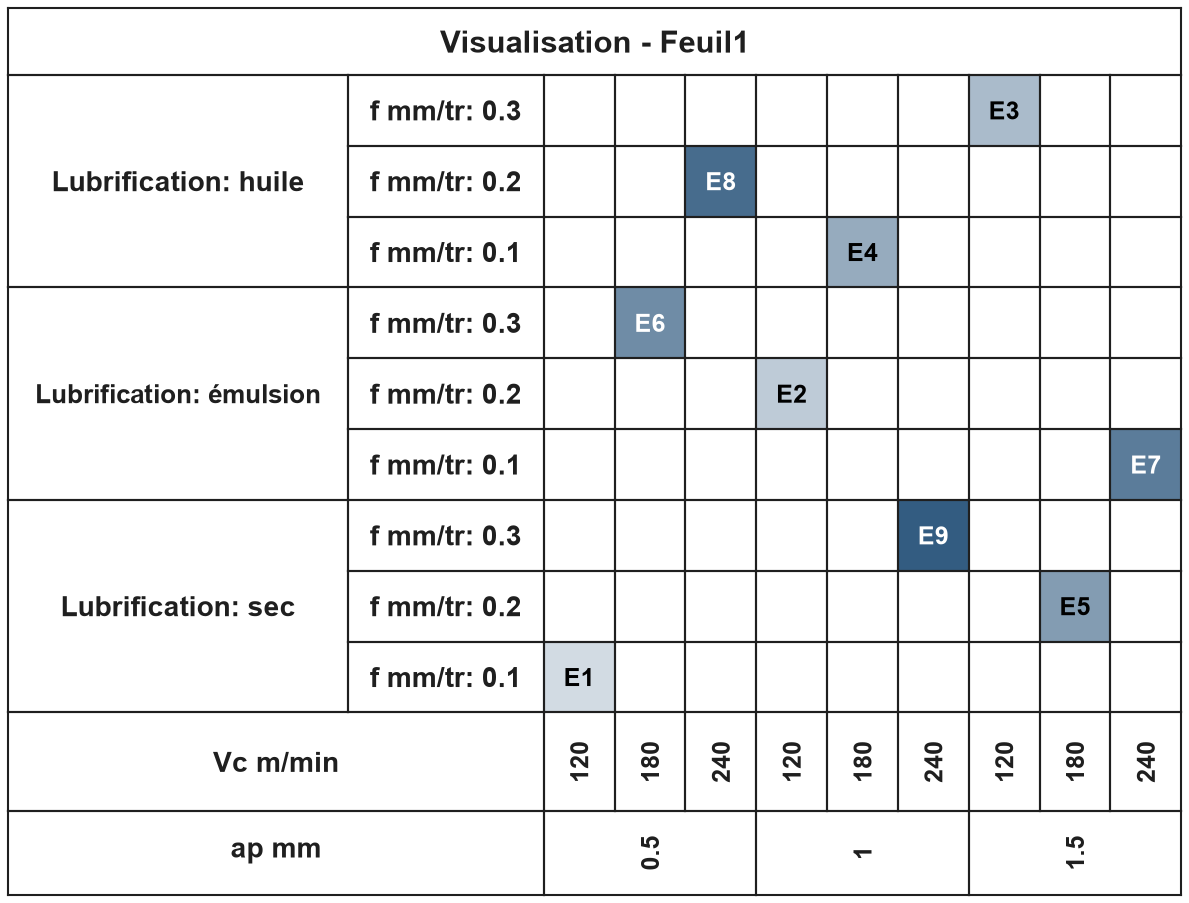
\includegraphics[width=\linewidth,height=0.25\textheight,keepaspectratio]{./_FIG/FIG_Partie_00/tournage_defaut.png}
\begin{lstlisting}[style=dimCode,numbers=none,basicstyle=\ttfamily\footnotesize,xleftmargin=0pt,breakatwhitespace=false,breakindent=0pt,keepspaces=true]
Style()
\end{lstlisting}
\raggedright\footnotesize Dégradé blanc vers bleu, sans légende supplémentaire. Le tableau et les axes restent identiques.
\end{column}
\begin{column}{0.32\textwidth}
\centering\textbf{Cividis}\\[0.2em]
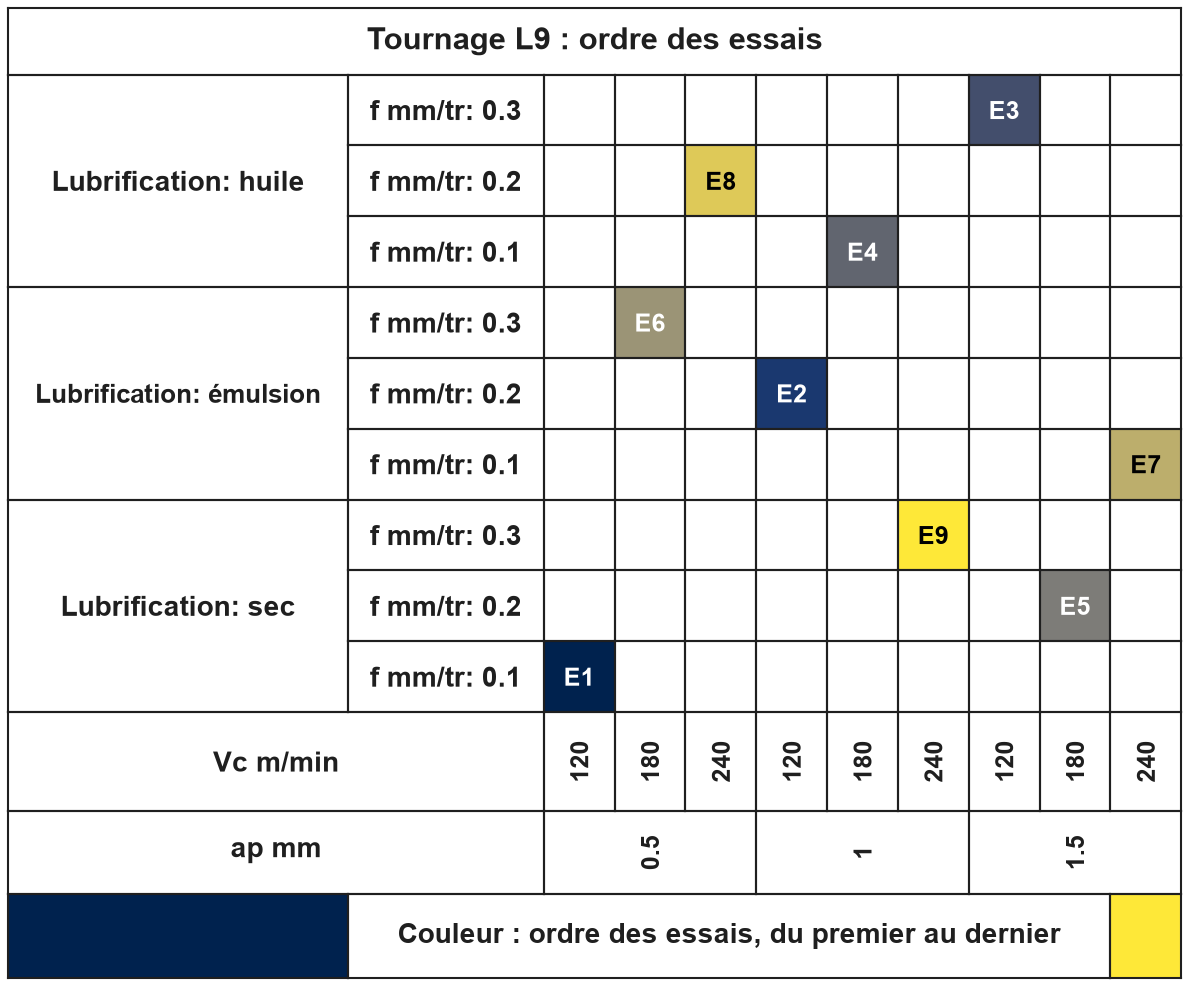
\includegraphics[width=\linewidth,height=0.25\textheight,keepaspectratio]{./_FIG/FIG_Partie_00/tournage_cividis.png}
\begin{lstlisting}[style=dimCode,numbers=none,basicstyle=\ttfamily\footnotesize,xleftmargin=0pt,breakatwhitespace=false,breakindent=0pt,keepspaces=true]
Style(
  palette="cividis",
  legend=True,
  title="Tournage L9 : "
        "ordre des essais")
\end{lstlisting}
\raggedright\footnotesize Palette lisible par les daltoniens ; la légende explique le rang.
\end{column}
\begin{column}{0.32\textwidth}
\centering\textbf{Personnalisé}\\[0.2em]
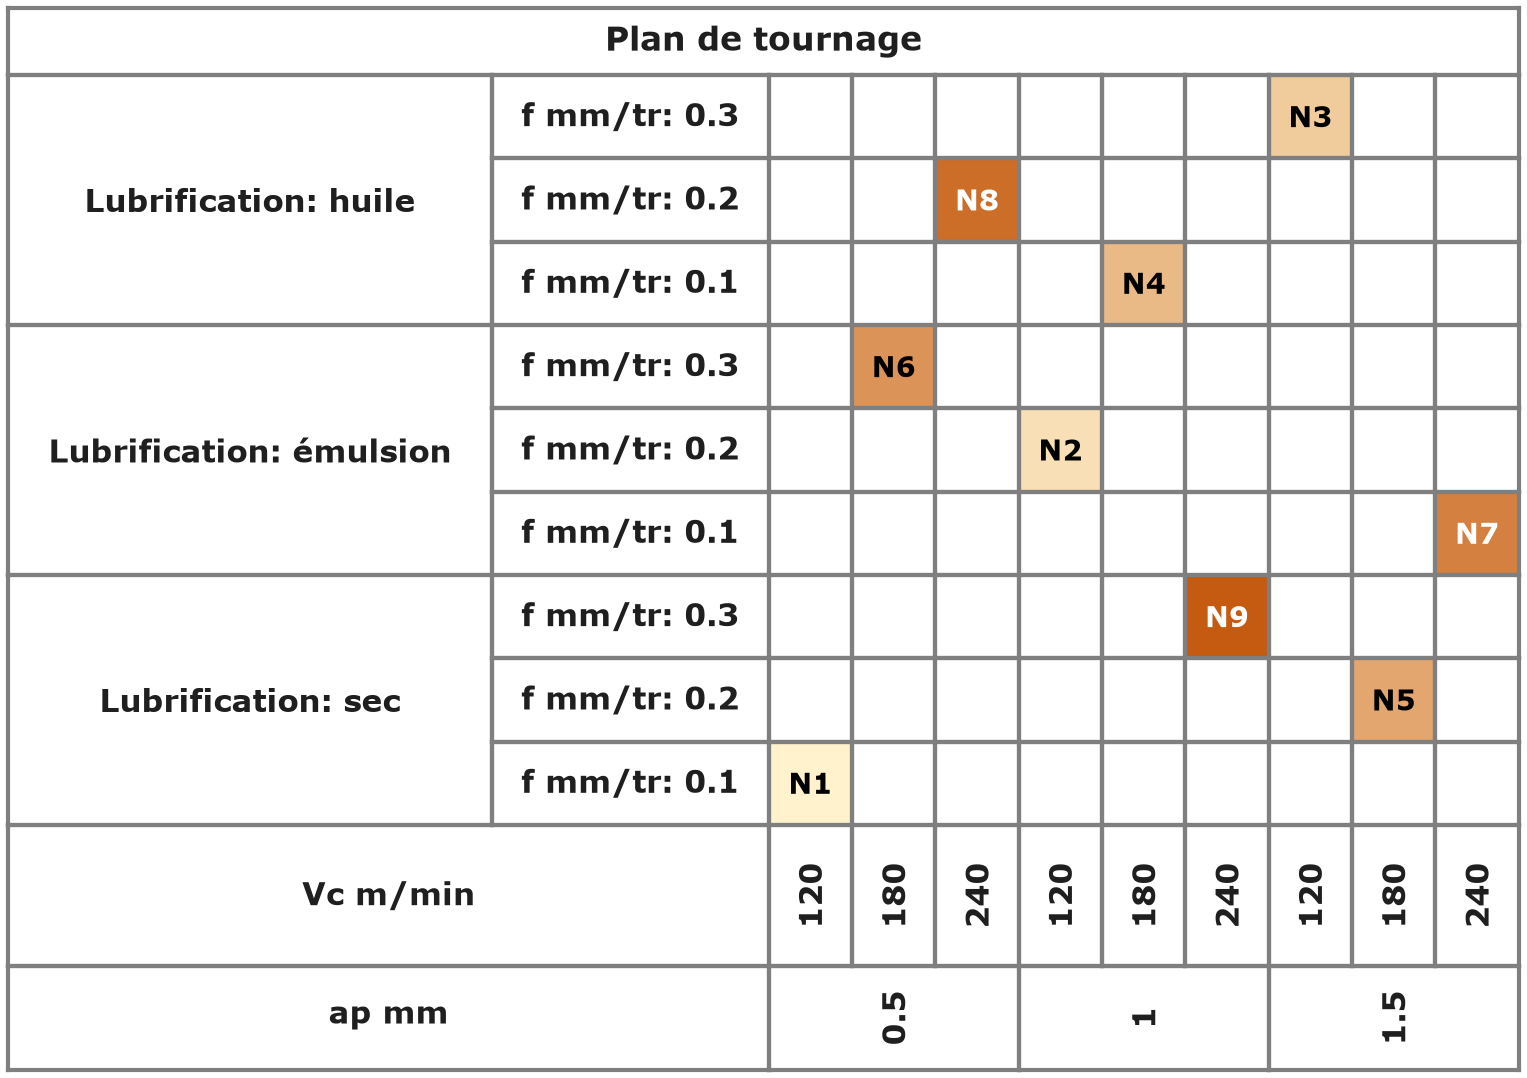
\includegraphics[width=\linewidth,height=0.25\textheight,keepaspectratio]{./_FIG/FIG_Partie_00/tournage_perso.png}
\begin{lstlisting}[style=dimCode,numbers=none,basicstyle=\ttfamily\footnotesize,xleftmargin=0pt,breakatwhitespace=false,breakindent=0pt,keepspaces=true]
Style(
  palette=("FFF2CC","C55A11"),
  font_family="Verdana",
  font_size=11,cell_size=40,
  line_color="7F7F7F",
  line_style="medium",
  run_prefix="N",
  title="Plan de tournage",
  label_scale=1.3)
\end{lstlisting}
\end{column}
\end{columns}
}
\note{Importer Style depuis dim2dir. Paramètres exacts des figures fournies, vérifiés dans le script de création de ces figures. label_scale réserve davantage d'espace à Verdana. Le défaut de legend reste False dans le rendu personnalisé.}
\vfill
\end{frame}

\begin{frame}[t]{Choisir la sortie et connaître les limites}
% [DEVELOPPE: défauts, limites et résultat]
\vfill
{\relscale{0.9}
Sans \texttt{outputs} : un classeur donne XLSX, PNG et PDF ; un DataFrame donne seulement PNG. Sans \texttt{output\_dir}, un DataFrame retourne les octets (\texttt{Result.data["png"]}) ; sinon \texttt{Result.files} liste les chemins. \texttt{Result.report} résume en texte ; \texttt{report=True} ajoute un JSON.
\begin{center}
\begin{tabular}{@{}lll@{}}
\toprule
\textbf{Champ de Limits} & \textbf{Défaut} & \textbf{Dépassement}\\
\midrule
\texttt{max\_cells} & \numprint{90000} & \texttt{visualize} : \texttt{skipped}\\
\texttt{max\_pixels} & \numprint{60000000} & \texttt{visualize} : \texttt{skipped}\\
\texttt{max\_runs} & \numprint{20000} & \texttt{Dim2DirError}\\
\texttt{excel\_timeout\_s} & 120 secondes & Erreur Excel ou repli en \texttt{auto}\\
\bottomrule
\end{tabular}
\end{center}
Relever \texttt{max\_cells} ne supprime pas les limites d'Excel (\numprint{16384} colonnes, \numprint{1048576} lignes). \texttt{max\_pixels} protège aussi PDF et SVG. \texttt{Result} n'a pas d'attribut de statut : \texttt{skipped} figure dans les rapports.
}
\note{Limits est immuable et validé. figure lève Dim2DirError si le rendu dépasse les limites. Le moteur Excel exige Windows et Excel de bureau ; le SVG utilise matplotlib. Un export ignoré laisse disponibles les fichiers déjà produits. visualize renvoie le statut dans le résumé Result.report et le JSON si report=True, et les raisons dans Result.warnings. Max_cells : pas d'image, classeur demandé avec message de refus ; max_pixels : pas d'image, classeur demandé conservé. project calcule la projection sans grille dense malgré max_cells. Les dépassements max_runs interrompent aussi project. Délai COM : engine=excel lève Dim2DirError ; engine=auto avertit et se replie sur matplotlib. in_memory=False exige output_dir pour un DataFrame.}
\vfill
\end{frame}

\begin{frame}[t]{Ce qu'il faut retenir}{Dans un programme Python}
\vfill
{\relscale{0.9}
\begin{mybox3}[yellow!8!white][Framajaune][Framajaune]{\textbf{Points clés}}
\begin{itemize}\itemsep5pt
\item \texttt{project} calcule la couverture sans produire de fichier.
\item \texttt{figure} retourne une figure pour le notebook ou l'application.
\item \texttt{visualize} livre les formats demandés, sur disque ou en mémoire.
\item \texttt{Style} personnalise le rendu sans changer les combinaisons essayées.
\item \texttt{Limits} protège les ressources ; lire les avertissements retournés.
\end{itemize}
\end{mybox3}
Le même appel traite un classeur ou un DataFrame. Préparer les facteurs, choisir la sortie et vérifier la couverture avant d'intégrer l'image à une application.}
\note{Les sorties ne prouvent ni l'optimalité statistique du plan, ni la qualité des mesures. Elles décrivent les combinaisons parmi les niveaux observés.}
\vfill
\end{frame}
